\RequirePackage{xcolor}
\documentclass[a4]{sciposter}
\usepackage{multicol,subfig,amsmath} % columnas, figuras, ecuaciones
\usepackage{graphicx,url,hyperref,doi}
\hypersetup{hidelinks} 
\usepackage[spanish]{babel}   
\usepackage[utf8]{inputenc}
\usepackage[sort&compress,numbers]{natbib}
\usepackage[font=small,labelfont=bf]{caption}
\usepackage[bottom]{footmisc}

\usepackage{tikz} % diagramas
\tikzstyle{elem} = [draw, rectangle, thick, minimum height=2em, minimum width=2em]
\tikzstyle{line} = [draw, thick, -stealth, shorten >=1pt]

\setlength{\parskip}{3pt} % espacio entre parrafos
\renewcommand{\arraystretch}{1.5} % altura de renglones de cuadros

\leftlogo[1]{img/UANL.png}
\rightlogo[1]{img/FIME.png} 

\title{Mejora de algoritmo de\\reconocimiento de emociones}
\author{Alexander Espronceda Gómez,\\Cecilia Jael Aguilar Aranda$^\dagger$,\\Satu Elisa Schaeffer}
\institute {Posgrado en Ingeniería de Sistemas}
\email{$^\dagger$cjaelaguilar@gmail.com}



\begin{document}

\conference{Verano Científico FIME UANL 2021}

\maketitle

\begin{abstract}
En este proyecto se busca incrementar el funcionamiento de un algoritmo de análisis de sentimientos en base a texto utilizando redes neuronales. Esto conlleva realizar modificaciones al código, aí como el aumento del dataset con el que se trabaja. El objetivo es realizar un chatbot capaz de reconocer patrones, determinar el sentimeinto mostrado por el usuario y actuar acorde a ello.
\end{abstract}

\begin{multicols}{2} 

\section{Introducción}

El objetivo principal de este proyecto es llevar a cabo diversos procesos que ayuden a que un algoritmo de análisis de sentimientos por medio de texto tenga un porcentaje de acierto más alto. Esto se logrará mediante búsqueda, análisis y filtrado de datos relevantes, así como también la actualización del algoritmo que está siendo utilizado actualmente.

\section{Antecedentes}

El algoritmo de análisis de sentimientos por medio de texto que se utiliza en este proyecto le corresponde a Alexander Espronceda Gómez, quien actualmente está escribiendo un paper al respecto \citep{chatbot}. Por lo tanto, este proyecto sólamente se enfoca en el mejoramiento de éste, y no en el proceso completo.
\begin{figure}
	\centering
	\captionsetup{type=figure}
	\setcounter{figure}{0}
	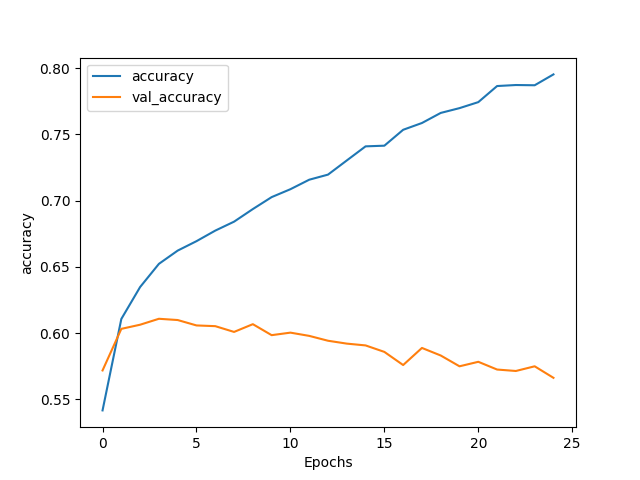
\includegraphics[scale=1.5]{img/Accuracy 2020-05_nofilter}
	\caption{Gráfica representativa del porcentaje de acierto del algoritmo, antes de aplicársele alguna mejora}
	
\end{figure}

\section{Estado de arte}

Qué han hecho los demás sobre este tema (citar a publicaciones
científicas, de preferencia publicadas en revistas que tengan DOI y
que por lo menos algunos sean de los últimos cinco años. Aquí se
suelen citar artículos como por ejemplo el trabajo de \citet{elisa} o
algo que se haya presentado en un congreso como \citet{ar}. A veces es
necesario definir algo matemático como por ejemplo
\begin{equation}
    f(x) = \sum_{i = 0}^\infty \sin(i x)
    \label{suma}
\end{equation}
para comunicar mejor lo que pasa.

Si una ecuación depende de otra, conviene mencionarlo de manera
explícita. Por ejemplo se puede poner $g(x) = \sqrt{f(x)}$, donde
$f(x)$ proviene de la ecuación \eqref{suma}.

Área de oportunidad: qué exactamente este trabajo contribuirá encima
de lo que ya existe.  {\textquestiondown}Qué tiene de
diferente/original/impacto?

\section{Solución propuesta}
La implementación se hizo en Python 3.7 \citep{python}, además de otras herramientas relacionadas con redes neuronales como Tensorflow 2.0.0 \citep{tensorflow}.



\subsection{Metodología}
Se comenzó por una búsqueda de datasets, utilizandose la librería NLTK \citep{nltk} para filtrar palabras que no aportan mucho significado al texto.

Se consideró mejor un enfoque generalista debido a que las diferentes etiquetas de sentimiento a analizar no estaban distribuidas de manera uniforme; por lo que los datos se clasificaron únicamente en \textit{"Bueno"},\textit{"Neutral"} y \textit{"Malo"}.

Se utilizó un algoritmo bidireccional STM con una activación de softmax de última capa. El léxico está limitado a 5000 elementos, y el largo máximo de cualquier frase después de ser filtrada es de 30 caracteres.

Durante la fase de entrenamiento, se utilizaron 25 epochs con un 75\% del dataset en un orden arbitrario, usando el 25\% restante como validación.

\begin{figure}
	\centering
	\captionsetup{type=figure}
	\setcounter{figure}{1}
	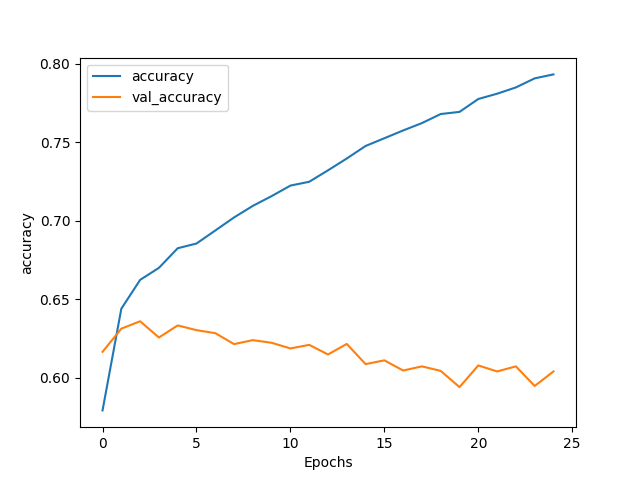
\includegraphics[scale=1.5]{img/Accuracy 2021-07.png}
	\caption{Gráfica representativa del porcentaje de acierto del algoritmo, después de aplicársele alguna mejora}
	
\end{figure}


Metodología, herramientas (qué en sí haces, cómo lo haces, con qué lo
haces).  La implementación se hizo en Python 3.9 \citep{python} y los
componentes se interconectan como muestra el diagrama de la figura
\ref{diag}.

\begin{figure}
\captionsetup{type=figure} % por culpa de sciposter
\setcounter{figure}{1} % por culpa de sciposter
\begin{center}
    \begin{tikzpicture}[]
      \matrix[row sep=0.5cm]{
      \node[elem] (n1) {Una cosa}; & & \node[elem] (n2) {Otra cosa}; \\
      & \node[elem] (n3) {Nueva cosa}; & \\
      };
     \draw [line] (n1) -- (n2);
     \draw [line] (n1) -- (n3);
     \draw [line] (n2) -- (n3);
    \end{tikzpicture}
\end{center}
\caption{Hay que explicar qué quieren decir los elementos de la figura.}
\label{diag}
\end{figure}

\section{Experimentos}

Diseño, reportaje y análisis de los resultados de los
experimentos. Por lo general se incluyen figuras como la figura
\ref{curvas}.

\begin{figure}
% por culpa de sciposter, hay que ajustar numeracion manualmente  
\setcounter{figure}{2} 
\captionsetup{type=figure} % por culpa de sciposter
\begin{center}
   \end{center}
    \caption{Hay que explicar qué quieren decir los elementos de la figura.}
    \label{curvas}
\end{figure}

Además es muy común incluir cuadros de datos, como por ejemplo el cuadro \ref{data}.

\begin{table}
\setcounter{table}{0} % por culpa de sciposter
\captionsetup{type=table} % por culpa de sciposter
\caption{Aquí explicas cómo interpreta el cuadro.}
\label{data}
\begin{center}
\scalebox{0.9}{\begin{tabular}{|r|c|l|}
    \hline
         \multicolumn{1}{|c|}{\rotatebox{90}{\bf Valor}}
         & \multicolumn{1}{|c|}{\rotatebox{90}{\bf Parámetro}}
         & \multicolumn{1}{|c|}{\rotatebox{90}{\bf Descripción\phantom{m}}} \\
         \hline
         0.23 & $x$ & algo \\
         \hline
         2.34 & $y$ & demo \\
        \hline
    \end{tabular}}
\end{center}
\end{table}

\section{Conclusiones}

Se ha logrado un aumento en la precisión de reconocimiento de emociones, se espera realizar más modificaciones para mejorar el algoritmo y en un futuro implementarlo para su uso.

\paragraph{Agradecimientos}

{\small Agradecemos a la dra. Elisa Schaeffer por su apoyo en la realización del póster, además de el PROVERICYT y Delfín al dar la oportunidad de participar en el Verano de Investigación Científica y Tecnológica 2021 y proporcionar una beca.
El póster se preparó con \url{https://www.overleaf.com/}.}

\end{multicols}

\bibliography{poster}
\bibliographystyle{plainnat}

\end{document}
